% \chapter{Determining how to parse a formal language}

\section{Introduction}
% About how compilers work, three parts. the lit review focus on parsing part

\newpage
\section{Language Parsing Design}

\subsection{Determining how to parse the syntax of a language}

A formal language is defined as a set of strings of symbols for use in situations where a natural language(\emph{English}) isn't suitable eg. Mathematics, and Computer programming. Where each symbol has precise semantic, and syntactic relation to each other. Writing formal grammar rules uses a set of finite ``\emph{productions}''. Productions, are rules that signify substitution of symbols within a string, there are typically three symbols when writing productions in formal grammars.

\begin{description}
    \item[\emph{Terminal Symbols}] Symbols which cannot be substituted any further, an example of this in programming languages is single number digits(0-9). Terminal symbols are represented by lowercase letters.
    
    \item[\emph{Nonterminal Symbols}] Symbols which can be reduced further using productions. For example as in \ref{fig:formalGrammar} $A \rightarrow a\ |\ aA$ is a nonterminal rule, as \emph{A} needs to be substituted into either \emph{a}, or \emph{aA}. Nonterminal symbols are represented by uppercase letters.

    \item[\emph{Start Symbol}] is a special Nonterminal symbol signifying the start of a string. Start symbols are represented by a uppercase S, or an Uppercase S with a subscript s eg. $S_s$, in order to signify it is different from a Nonterminal \emph{S} symbol.
\end{description}


Productions rules are used show how a compiler will take strings, and convert them into tokens. The tokens are sorted into a hierarchy that can be used by the next stage of the compiler. The \emph{|}, known as the vertical bar or ``pipe'' symbol is just used to symbolise a grouping of rules applying to the same rule.

\begin{figure}[ht!]
    \begin{align*}
    S_s &\rightarrow AB\ |\ CC \\
    A &\rightarrow a\ |\ aA \\
    B &\rightarrow bc\ |\ bBc \\
    D &\rightarrow ab\ |\ aDb \\
    C &\rightarrow c\ |\ cC \\
    \end{align*}
    \caption{Formal grammar syntax, example from \autocite{ParseTech}}
    \label{fig:formalGrammar}
\end{figure}

\subsection{Chomsky hierarchy within formal languages}

When parsing a string as a way to meaningfully turn the language into meaningful data models, \autocite{Chomsky} talks about the need of structured models, rather than using probabilistic models like Markov Chain. Markov chain is a model where the data model changes from different states, based solely on it's most recent state. \autocite{Chomsky} showcases this with the famous example: \\\\ \centerline{``\emph{Colorless green ideas sleep furiously}''} \\

A sentence which is not a semantically valid sentence, but is grammatically correct. In \autocite{Chomsky} he defined what is now known as \emph{\hierarchy{}}, which defines formal languages into four types(Type 0 - 4). As shown in Figure \ref{fig:Chomsky} each type is a subset of the previous. All of Type 4, can be a Type 3, but not all of Type 3 can be Type 4, so multiple rules can describe the same language depending on it's syntax.
\clearpage
\begin{figure}[h]
    \centerline{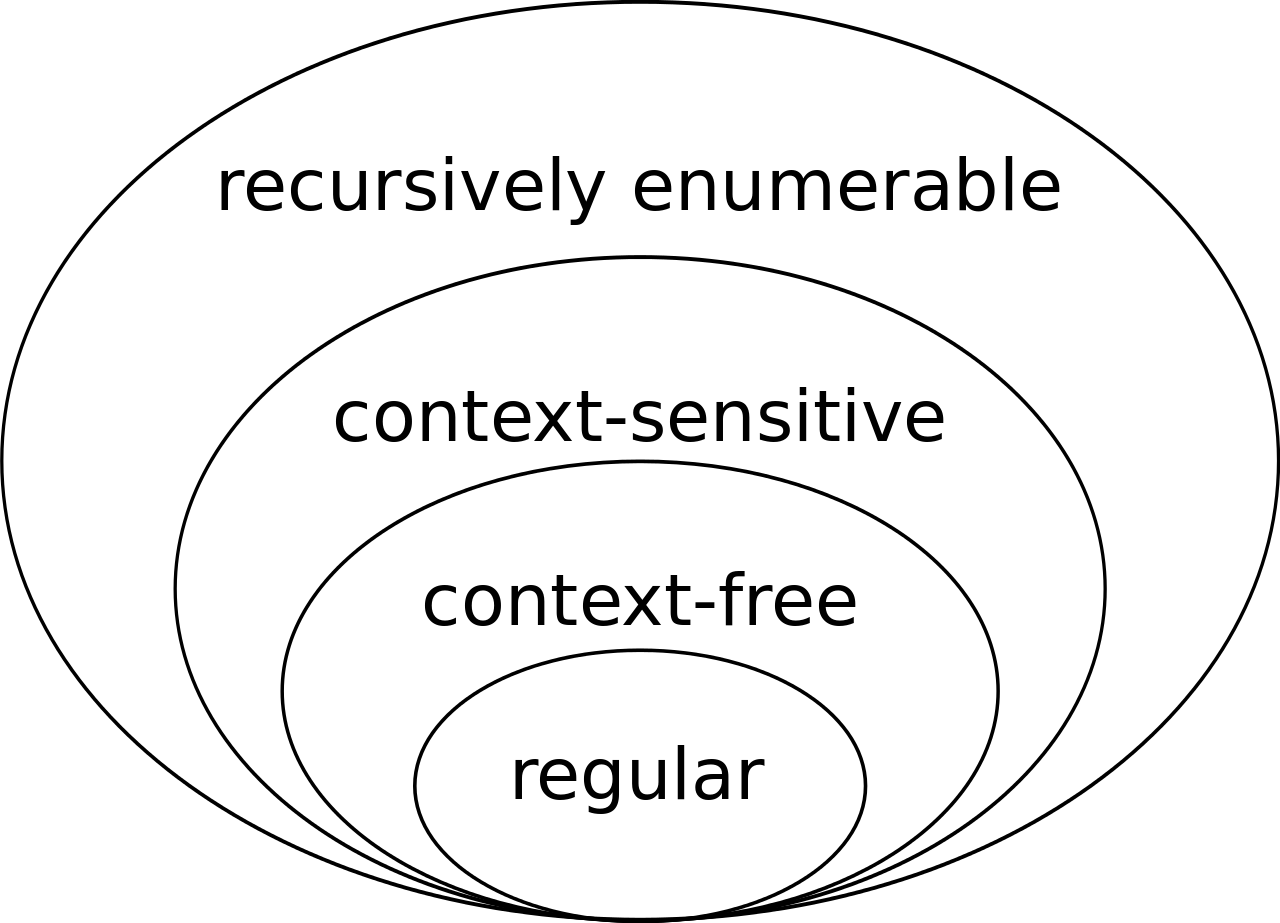
\includegraphics[width=0.5\linewidth]{img/Chomsky.png}}
    \caption{\hierarchy{}, by J. Finkelstein}
    \label{fig:Chomsky}
\end{figure}
\begin{description}
    \item[Type 0] Also known as \emph{recursively enumerable} languages. This is the the parent of all following languages. Every language in the Chomsky hierarchy is also a recursively enumerable. Recursively enumerable is a generalised, and can have unclear hierarchy, due to it's lack of limitations.
    \item[Type 1] Also known as \emph{context-sensitive} languages. Meaning only one of the nonterminal characters on the left hand side can be replaced. This allows for a much clearer hierarchy within the parse tree.
    \item[Type 2] Also known as \emph{context-free} languages. context-free is similar to context sensitive, except there is always only one Nonterminal Symbol on the left hand side. This prevents children in the parse tree to have star patterns with multiple parents pointing to the same child, which then points to multiple children within the parse tree. This is known as a \emph{pure} hierarchy. This is a the language type most programming languages fall under, with few exceptions(\emph{C++}).
    \item[Type 3]  Also known as \emph{regular} languages. Regular languages are languages defined by \emph{regular expressions} rather than regular grammar like seen previously. Regular expressions are often used when the lexical rules of a language are simple, and don't require powerful notations like grammars. Regular expressions are also much more concise in the expressing notation, than it's grammar equivalents. However regular expressions cannot describe nested structures within the language, which can be very limiting \autocite{DragonBook}.
\end{description}

\subsection{Using \hierarchy{} \\within a compiler}
When discussing about parsing a programming language, it is important to differentiate between the syntax of the language, and the \emph{semantics} of the language. As confusion between the two can lead an individual to believe a language is one type, when it is actually a subset. As \autocite{DragonBook} shows, compilers when parsing language have a lexical analyser, which would group characters into much more meaningful sequences known as \emph{lexemes}. Lexemes are then converted into a tokens commonly in the form of a key, value pairing.\\\\ \centerline{(\emph{token-name}, \emph{attribute-value})} \\

Raw symbols like digits, or mathematical symbols(\emph{+,-,/,*}) are mapped into their token-name equivalents. Where as variables, the compiler will map the token-name to a token representing that it is an identifier eg. \emph{id, ident, identifier}. The compiler will then assign the attribute-value to number representing it's key in the Symbol-Table. The Symbol-Table is designed to contain much more concrete information about the token, such as it's name, and it's type eg. \emph{int, float, double, string}. The set of tokens is then passed to the syntax analyser. The syntax analyser will only look at the token-name getting only a vary abstract representation of the code, and can only report syntactical errors such as using wrong keywords, or having incorrect mathematically expressions eg $int x  = 1 + - + 1;$. As the syntax analyser goes through each token it builds a parse tree, showing the relationship of the tokens as seen in \ref{fig:AST}. It is solely within the syntax analyser that defines the language type of the programming language.
\begin{figure}[ht!]
    \centering
    \begin{tikzpicture}
        \tikzset{every tree node/.style={align=center,anchor=north}}
        \Tree[.= [.x \textit{id} ] 
                 [.+  
                     [.1 ] 
                     [.+ [.- ]  
                         [.+ {} 
                             [.1 ] 
                         ] 
                        ]  
                     ]  
                 ]  
             ] 
    \end{tikzpicture}
    \caption{An Abstract Syntax Tree.}
    \label{fig:AST}
\end{figure}

The semantics of the language are analyser. This is shown clearly in \ref{fig:InvalidC}. Where when run through a C compiler the compiler will print out ``\emph{error: \lq{}x\rq{} undeclared (first use in this function)}''. 

\begin{figure}[ht!]
    \begin{verbatim}
                int main() {
                    x++;
                    int x = 1;
                    return 0;
                }
    \end{verbatim}
    \caption{C code with valid syntax, but invalid semantics.}
    \label{fig:InvalidC}
\end{figure}

This could lead an individual that the parser must be context-sensitive, as the compiler knew that ``\emph{x}'' was being used before it existed. However the compiler could be using a parsing grammar that is context-free, and the semantic analyser is what determined that the code written was invalid. Using the methods laid out in \autocite{DragonBook} the parser of a compiler would commonly not try structure the strings into a data model, and also interpret the meaning of the code.



\newpage
\section{Conclusion}
\newpage
